\documentclass[10pt,a4paper]{article}
\usepackage[T1]{fontenc}
\usepackage[utf8]{inputenc}
\usepackage[polish]{babel}
\usepackage{lmodern,graphicx,booktabs,float,siunitx,enumitem,microtype,caption}
\usepackage[margin=2cm]{geometry}
\sisetup{output-decimal-marker={,},group-digits=none}
\graphicspath{{images/}}
\setlength{\parindent}{0pt}
\setlength{\parskip}{4pt}
\setlength{\intextsep}{8pt}
\setlist[enumerate]{leftmargin=*,itemsep=2pt,topsep=3pt}
\captionsetup{font=small}
\InputIfFileExists{author.tex}{}{%
  \newcommand{\StudentNames}{Autorzy do uzupełnienia}%
  \newcommand{\StudentIndices}{Indeksy do uzupełnienia}%
  \newcommand{\LabGroup}{Grupa 2, 15:15--16:55}%
}
\newcommand{\FullRtwo}{\num{0.666324}}
\newcommand{\CleanRtwo}{\num{0.999993}}
\newcommand{\FullSlope}{\num{0.499727}}
\newcommand{\CleanSlope}{\num{0.345390}}
\newcommand{\FullIntercept}{\num{3.002455}}
\newcommand{\CleanIntercept}{\num{4.005649}}
\newcommand{\LowerBound}{\num{3.655}}
\newcommand{\UpperBound}{\num{10.575}}

\title{\vspace{-1.5cm}Regresja liniowa i kwartet Anscombe'a\\\large Ćwiczenie 1 -- Analiza danych eksperymentalnych}
\author{\normalsize\StudentNames\\\small Indeksy: \StudentIndices\quad |\quad \LabGroup}
\date{\small 20 października 2026}
\begin{document}
\maketitle
\vspace{-1cm}

\section*{Zadanie 1. Kwartet Anscombe'a}
W Pythonie i Excelu obliczyliśmy średnie, wariancje i korelacje dla czterech serii
po 11 obserwacji. Dopasowaliśmy proste $y=\beta_0+\beta_1x$ metodą najmniejszych
kwadratów. Podane wariancje mają dzielnik $n-1$.

\begin{table}[H]\centering\small
\begin{tabular}{lrrrrrr}
\toprule
Seria & $n$ & $\bar{x}$ & $\bar{y}$ & $s_x^2$ & $s_y^2$ & $r$ \\
\midrule
I & 11 & \num{9.000000} & \num{7.500909} & \num{11.000000} & \num{4.127269} & \num{0.816421} \\
II & 11 & \num{9.000000} & \num{7.500909} & \num{11.000000} & \num{4.127629} & \num{0.816237} \\
III & 11 & \num{9.000000} & \num{7.500000} & \num{11.000000} & \num{4.122620} & \num{0.816287} \\
IV & 11 & \num{9.000000} & \num{7.500909} & \num{11.000000} & \num{4.123249} & \num{0.816521} \\
\bottomrule
\end{tabular}

\caption{Statystyki i współczynniki regresji dla czterech serii.}
\end{table}
\begin{figure}[H]\centering
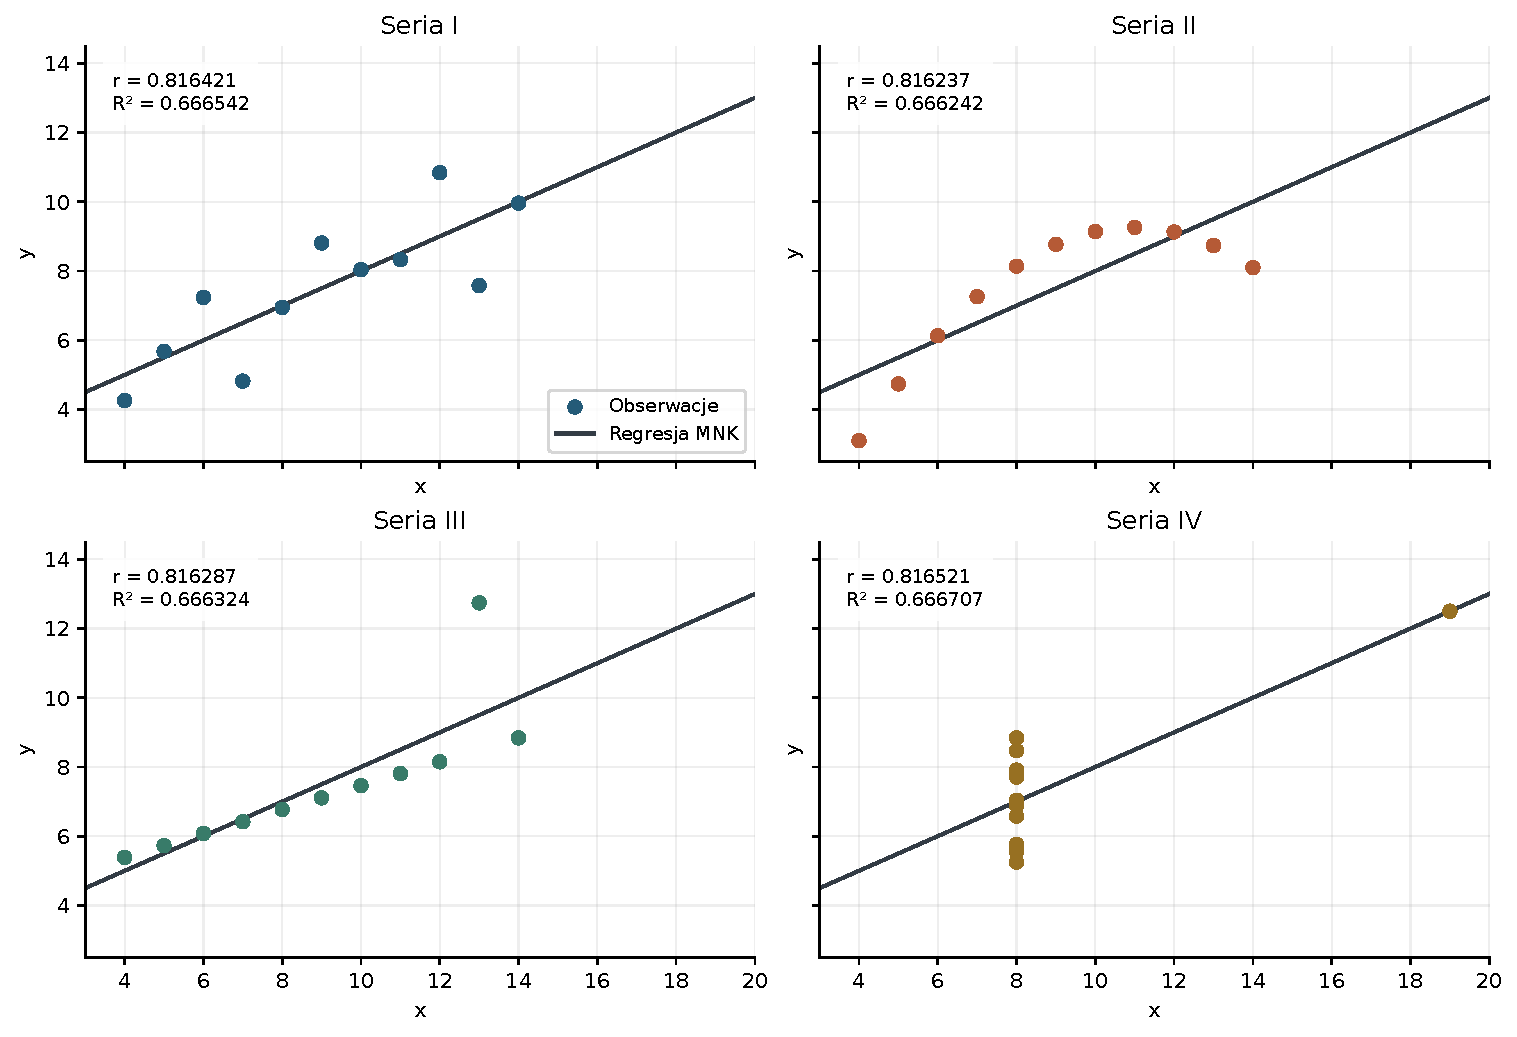
\includegraphics[width=0.94\linewidth]{anscombe_regression.pdf}
\caption{Dane i proste regresji. We wszystkich panelach zastosowano te same zakresy osi.}
\end{figure}
\textbf{Wnioski}
\begin{enumerate}
\item Średnie, wariancje i współczynniki regresji są niemal takie same, mimo różnych układów punktów.
\item Seria I przedstawia w przybliżeniu zależność liniową z rozrzutem wokół prostej.
\item Seria II ma wyraźnie zakrzywiony przebieg, którego prosta nie odtwarza.
\item W serii III jeden punkt odstający zmienia położenie dopasowanej prostej.
\item W serii IV dziesięć punktów ma $x=8$. Wynik regresji silnie zależy od jedynego punktu z $x=19$.
\item Podobna korelacja, około 0,816, nie wystarcza do oceny danych. Trzeba obejrzeć wykres.
\end{enumerate}

\clearpage
\section*{Zadanie 2. Zapis danych i usunięcie punktu odstającego}
Te same 44 obserwacje z zadania 1 zapisaliśmy w formatach CSV, JSON i XML.
Pliki mają kodowanie UTF-8; ich rozmiary zmierzyliśmy przed kompresją.
\begin{table}[H]\centering\small
\begin{tabular}{lrr}
\toprule
Plik & Rozmiar [B] & Względem CSV \\
\midrule
\texttt{anscombe.csv} & 555 & \num{1.000} \\
\texttt{anscombe.json} & 1470 & \num{2.649} \\
\texttt{anscombe\_pretty.json} & 2527 & \num{4.553} \\
\texttt{anscombe.xml} & 3033 & \num{5.465} \\
\texttt{anscombe\_pretty.xml} & 3958 & \num{7.132} \\
\bottomrule
\end{tabular}

\caption{Rozmiary plików zawierających te same dane.}
\end{table}
CSV zapisuje tabelę w kolejnych wierszach. JSON zapisuje tutaj tablicę obiektów,
a XML -- rekordy opisane znacznikami.

\textbf{JSON.} Nawiasy \texttt{\{\}} oznaczają obiekt, a \texttt{[]} tablicę.
Klucze i napisy zapisuje się w podwójnych cudzysłowach. Dwukropek oddziela klucz
od wartości, a przecinek kolejne elementy. Wartościami mogą być m.in. liczby,
napisy, tablice, obiekty, \texttt{true}, \texttt{false} i \texttt{null}.
JSON jest często stosowany w API internetowych i plikach konfiguracyjnych.
Przykładowy rekord: \texttt{\{"series":"I","x":10.0,"y":8.04\}}.

\textbf{Punkt odstający.} W trzeciej serii zastosowaliśmy regułę IQR dla $y$:
obliczyliśmy kwartyle $Q_1$, $Q_3$ i ich różnicę IQR, a następnie oznaczyliśmy wartości
poza zakresem od $Q_1-1{,}5\,\mathrm{IQR}$ do $Q_3+1{,}5\,\mathrm{IQR}$.
Granice wyniosły \LowerBound{} i \UpperBound.
Reguła wskazała jeden punkt: $(13;12{,}74)$. Po jego usunięciu ponownie dopasowaliśmy prostą.
\begin{table}[H]\centering\small
\begin{tabular}{lrrrrr}
\toprule
Dane & $n$ & $\hat\beta_0$ & $\hat\beta_1$ & $R^2$ & RMSE \\
\midrule
Przed & 11 & \num{3.002455} & \num{0.499727} & \num{0.666324} & \num{1.118286} \\
Po & 10 & \num{4.005649} & \num{0.345390} & \num{0.999993} & \num{0.002756} \\
\bottomrule
\end{tabular}

\caption{Regresja przed usunięciem punktu i po jego usunięciu.}
\end{table}
\begin{figure}[H]\centering
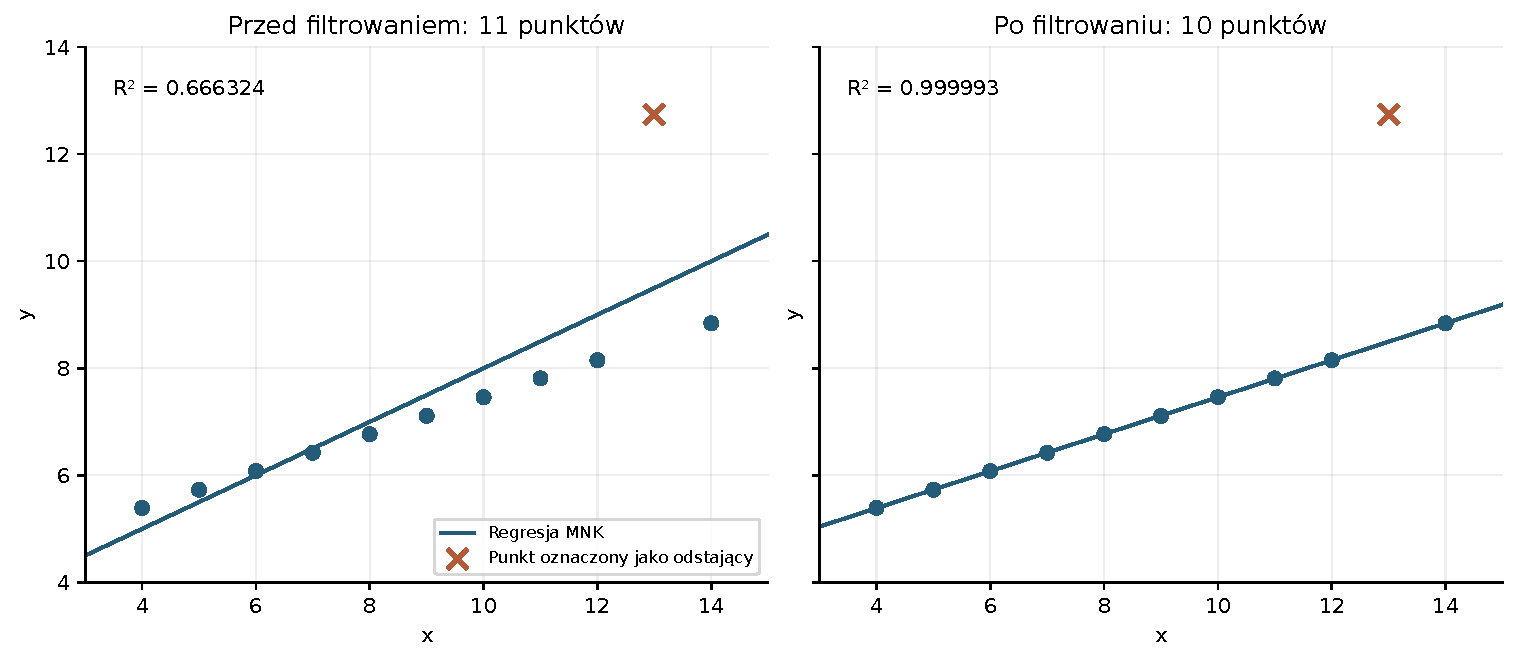
\includegraphics[width=0.94\linewidth]{outlier_comparison.pdf}
\caption{Porównanie serii III przed usunięciem punktu i po jego usunięciu.}
\end{figure}
\textbf{Wnioski}
\begin{enumerate}
\item CSV zajmuje najmniej miejsca, ponieważ nazwy kolumn zapisuje tylko raz.
\item JSON i XML mają większy narzut przez powtarzane klucze lub znaczniki, ale czytelnie opisują strukturę danych.
\item Wszystkie trzy formaty przechowują te same obserwacje. Różni się sposób ich zapisu.
\item Reguła IQR wskazuje dokładnie jeden punkt odstający: $(13;12{,}74)$.
\item Po jego usunięciu $R^2$ rośnie z \FullRtwo{} do \CleanRtwo. Pozostałe punkty są niemal współliniowe.
\item Lepsze dopasowanie po usunięciu punktu nie dowodzi błędu pomiaru. Warto zachować i porównać oba wyniki.
\end{enumerate}

\clearpage
\section*{Zadanie 3. Trzy serie z pliku CSV}
Wybraliśmy serię 1 oraz serie 9 i 10, po 142 obserwacje.
W Pythonie obliczyliśmy wymagane statystyki i dopasowaliśmy proste regresji.
Wyniki i wykresy umieściliśmy również w tym samym arkuszu Excel co pozostałe zadania.
\begin{table}[H]\centering\small
\begin{tabular}{lrrrrrrr}
\toprule
Seria & $\bar{x}$ & $\bar{y}$ & $s_x^2$ & $s_y^2$ & $r$ & $\beta_0$ & $\beta_1$ \\
\midrule
seria1 & \num{54.2633} & \num{47.8323} & \num{281.0700} & \num{725.5160} & \num{-0.0645} & \num{53.4530} & \num{-0.1036} \\
seria9 & \num{54.2673} & \num{47.8377} & \num{280.8980} & \num{725.2268} & \num{-0.0683} & \num{53.7970} & \num{-0.1098} \\
seria10 & \num{54.2687} & \num{47.8308} & \num{281.2074} & \num{725.5334} & \num{-0.0686} & \num{53.8095} & \num{-0.1102} \\
\bottomrule
\end{tabular}

\caption{Statystyki i współczynniki regresji dla wybranych serii. Wariancje mają dzielnik $n-1$.}
\end{table}
\begin{figure}[H]\centering
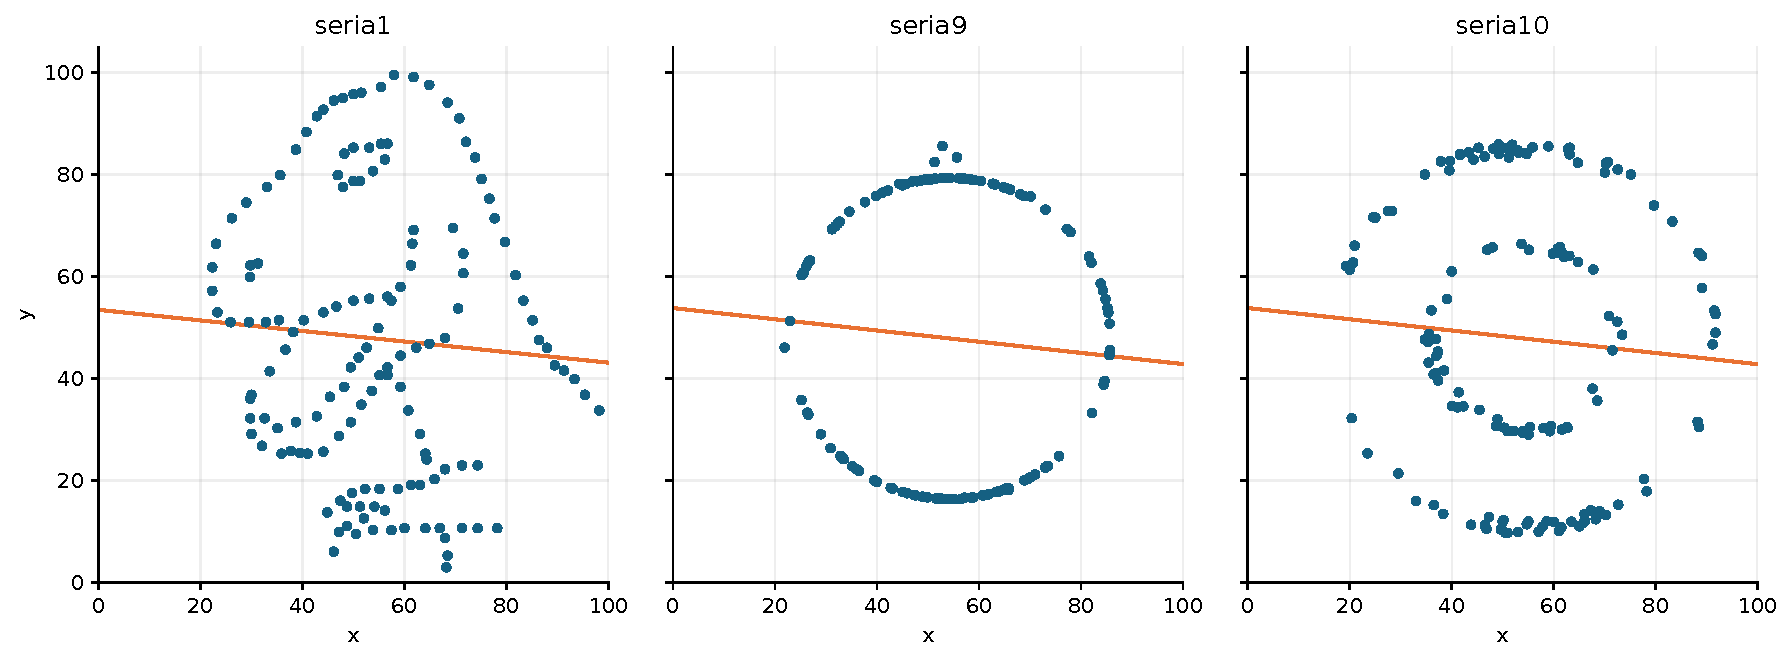
\includegraphics[width=\linewidth]{task3_regression.pdf}
\caption{Dane i proste regresji dla serii 1, 9 i 10.}
\end{figure}
\textbf{Wnioski}
\begin{enumerate}
\item Średnie są zbliżone: $\bar{x}\approx54{,}26$ i $\bar{y}\approx47{,}83$, mimo różnych kształtów danych.
\item Podobne wariancje, około 281 dla $x$ i 725 dla $y$, nie opisują rozmieszczenia punktów na płaszczyźnie.
\item Korelacje od około $-0{,}064$ do $-0{,}069$ oznaczają bardzo słabą zależność liniową.
\item Mała korelacja nie oznacza braku struktury: widać dinozaura, owalny pierścień i tarczę.
\item Prawie poziome proste nie odtwarzają widocznych kształtów. Sam model liniowy opisuje te dane słabo.
\item Wykresy ujawniają różnice, których nie widać w podobnych średnich, wariancjach i współczynnikach korelacji.
\end{enumerate}
\end{document}
